\newpage

\section{Additional Figures}\label{appFigures}

\textbf{
    In this section, we aim to verify that there is a reasonable range of scales, in terms of $\ell$, where the simulations are not dominated by numerical diffusion, but rather by correctly simulated turbulent cascades.
    Therefore, we offer some additional examples of which our VSFs look at different times and considering different analysis approaches.
    In particular, we focus on the standard analysis (Sects.~\ref{results:normal} and~\ref{discussion:normal}, Figs.~\ref{pic:appFigures:examples_with_threshold_s_vs_l} and~\ref{pic:appFigures:examples_with_threshold_sl_vs_l}), the density threshold-less scenario (Sects.~\ref{results:densthres} and~\ref{discussion:densthres}, Figs.~\ref{pic:appFigures:examples_without_threshold_s_vs_l} and~\ref{pic:appFigures:examples_without_threshold_sl_vs_l}), and the impact analysis of different Jeans refinement levels (Sects.~\ref{results:refinement} and~\ref{discussion:refinement}, Figs.~\ref{pic:appFigures:examples_jeans_s_vs_l} and~\ref{pic:appFigures:examples_jeans_sl_vs_l}).
}

\textbf{
    The figures are similar to the examples shown in Fig.~\ref{pic:results:vsf_example}, but with data from all three clouds and at three different snapshots during the simulations.
    The straight lines within the plots indicate the power-law relation that we have fitted onto the VSFs within the range of $\ell\,\leq$~8~pc.
}

\rc{continue?}
 	
\begin{figure*}
    \centering
    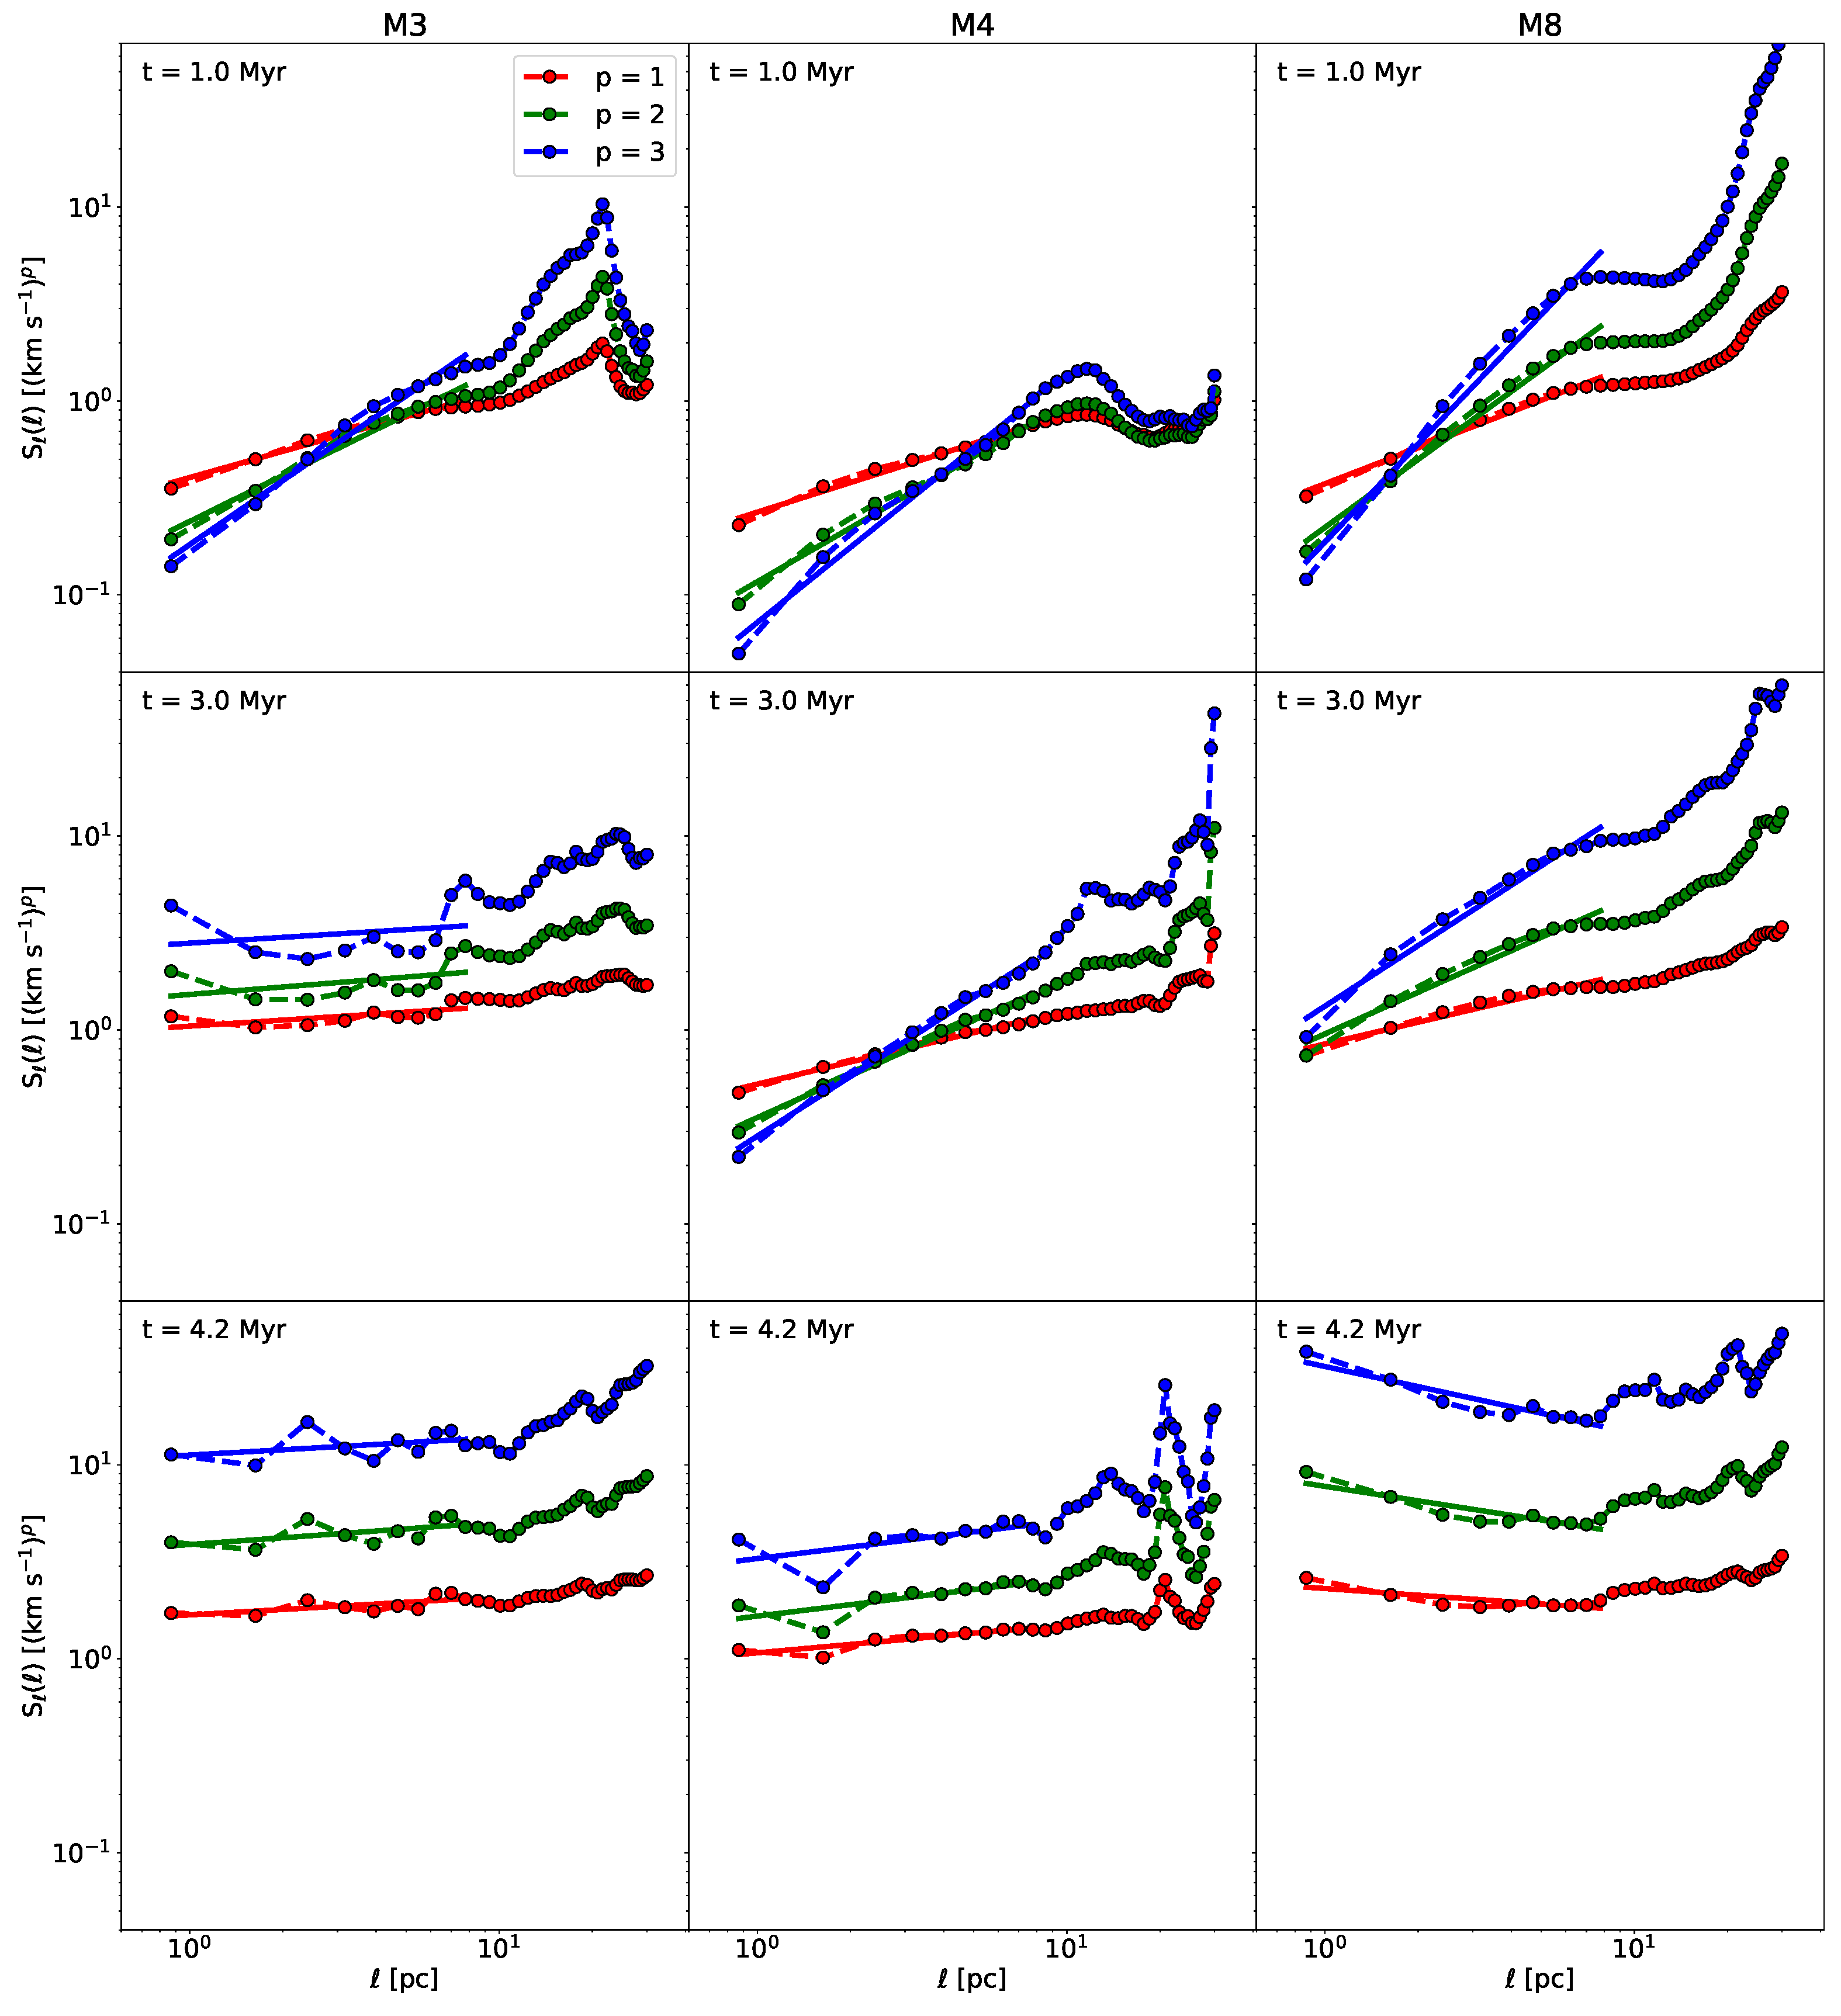
\includegraphics[width=\textwidth]{app_examples_wthres_s_l.pdf}
    \caption{
        The figures show additional examples of VSFs, based on data with density threshold, of (\textit{left} to \textit{right}) \texttt{M3}, \texttt{M4}, and \texttt{M8} as function of lag scale $\ell$ and order $p$. 
        The examples are given for three different time steps, namely (\textit{top} to \textit{bottom}) t~=~1.0~Myr, 3.0~Myr, and 4.2~Myr.
        The dots (connected by dashed lines) show the values computed from the simulations. 
        The solid lines represent the power-law relation fitted to the respective structure functions.
    }
    \label{pic:appFigures:examples_with_threshold_s_vs_l}
\end{figure*}
 	
 	
\begin{figure*}
    \centering
    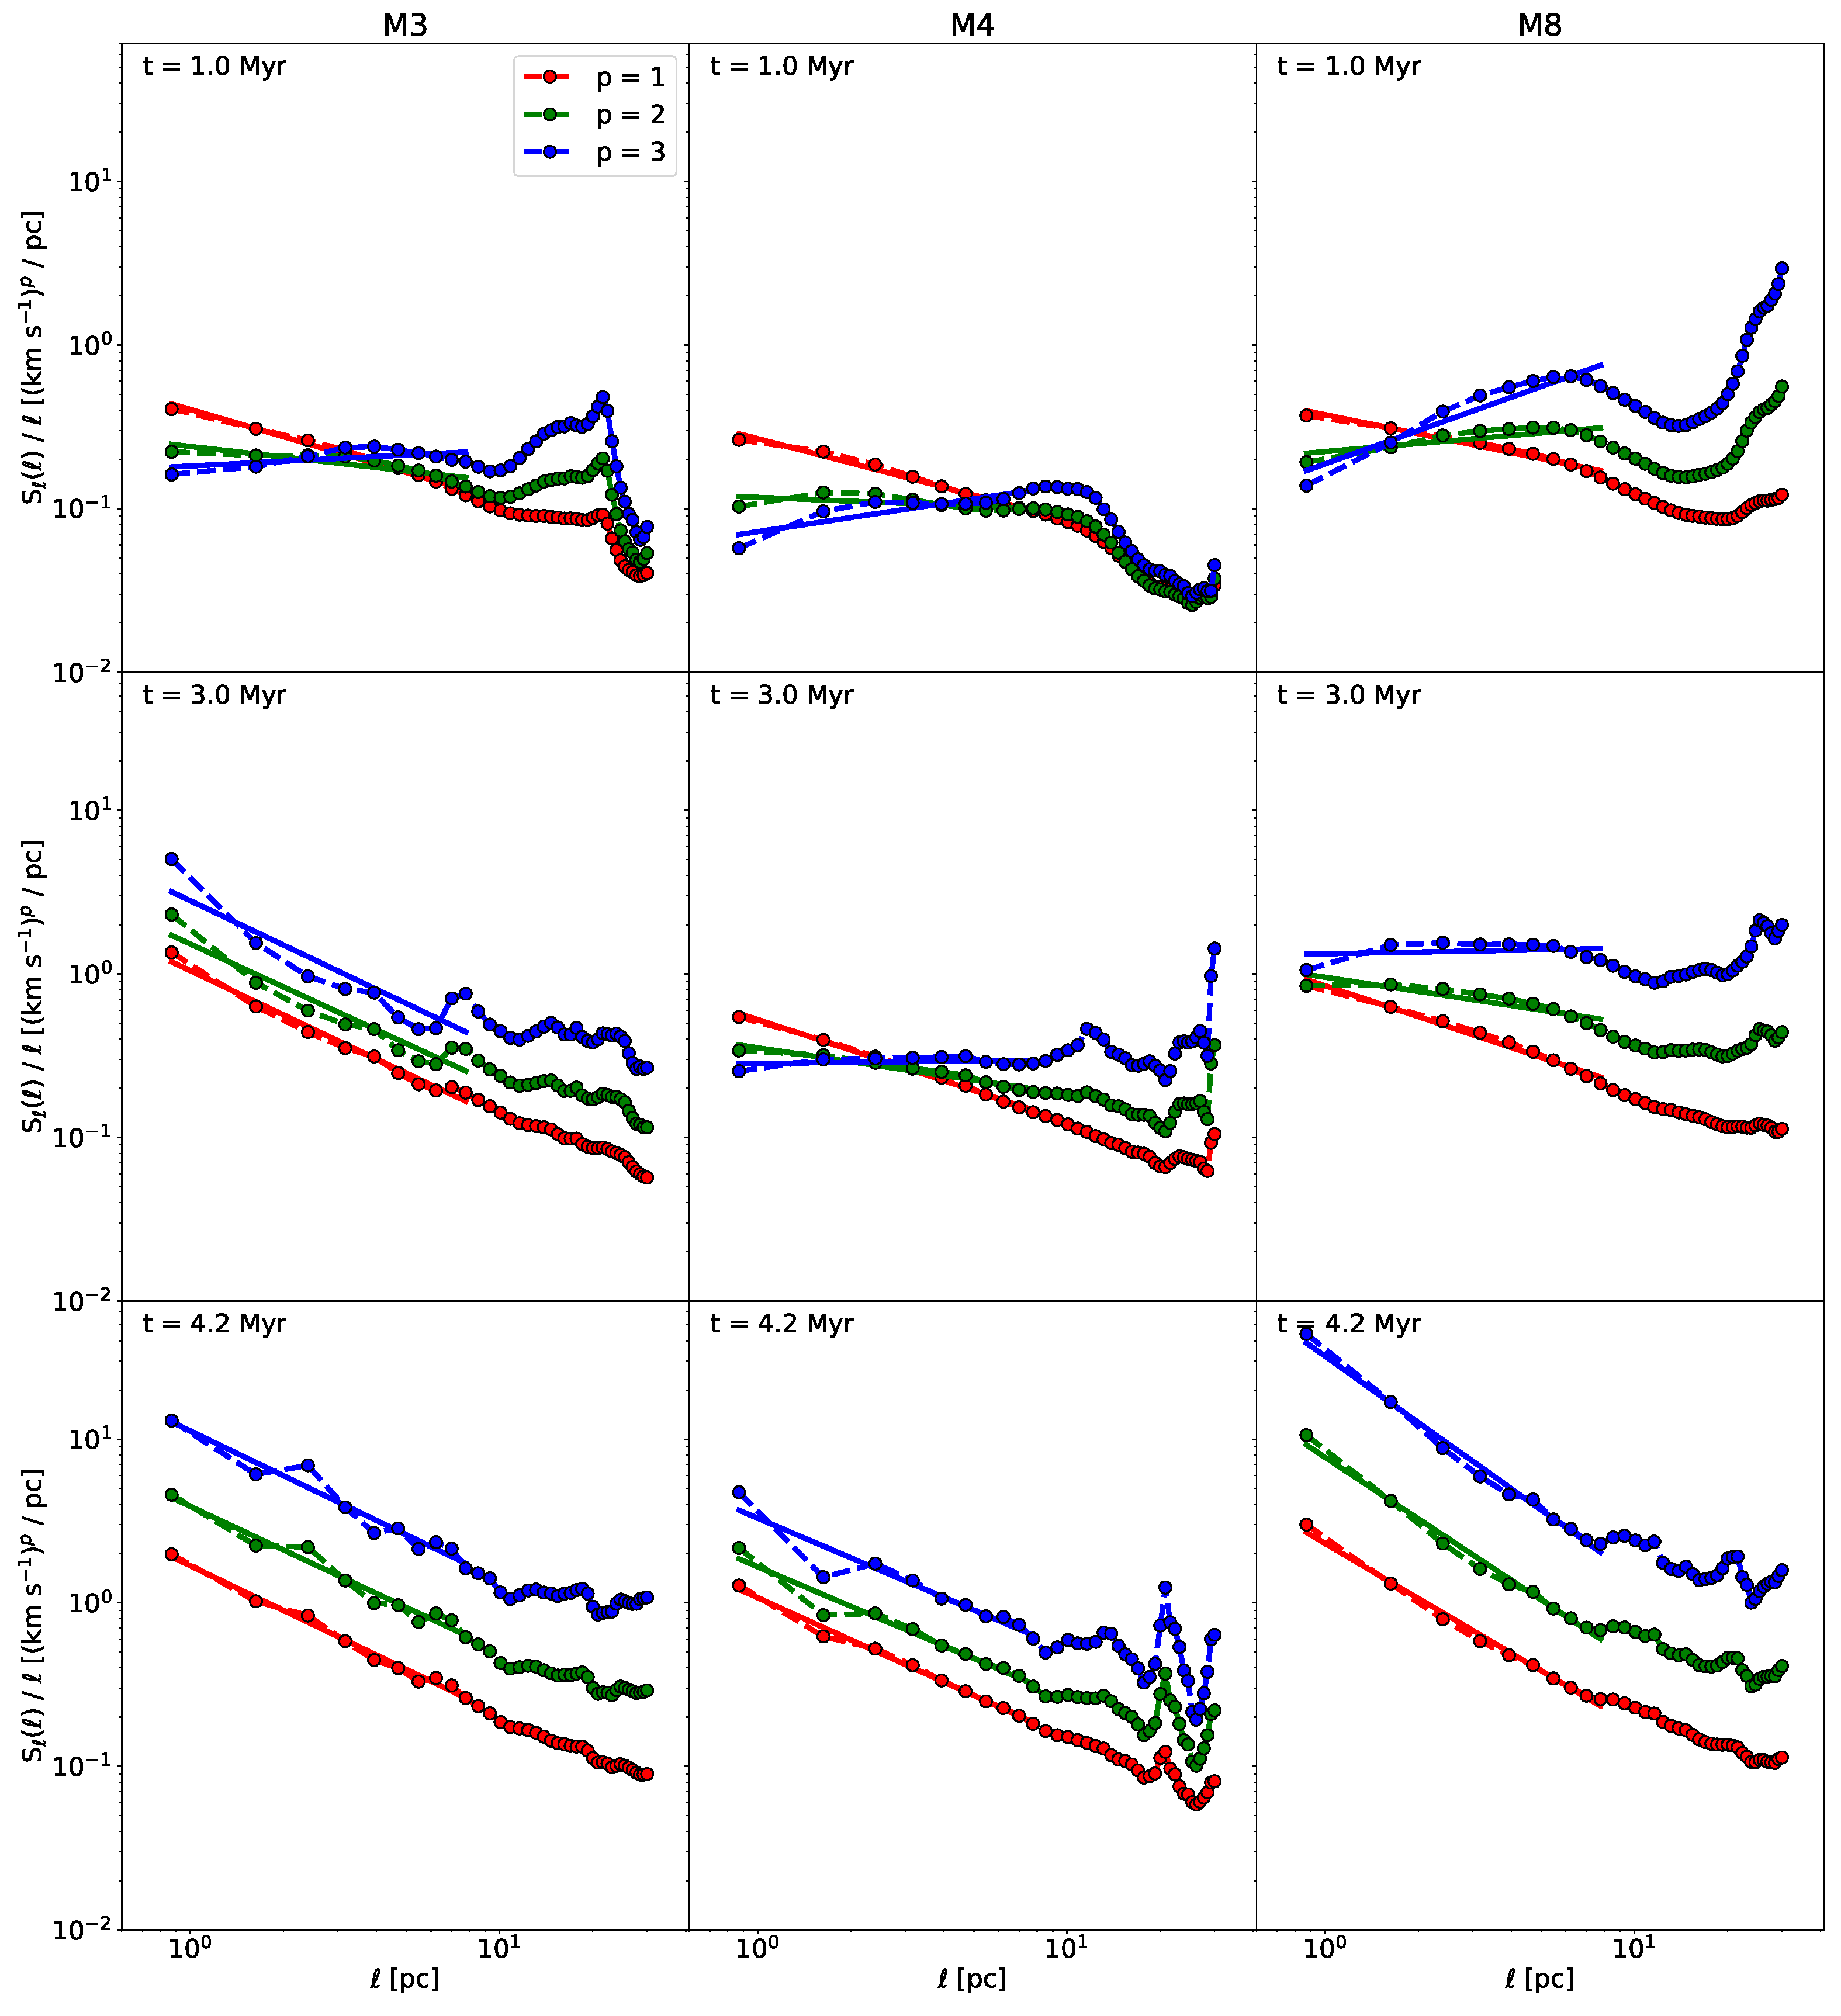
\includegraphics[width=\textwidth]{app_examples_wthres_sl_l.pdf}
    \caption{
        As Fig.~\ref{pic:appFigures:examples_with_threshold_s_vs_l}, but plotting the relation between S$_{\ell}$ / $\ell$ as function of lag scale $l$ and order $p$.
    }
    \label{pic:appFigures:examples_with_threshold_sl_vs_l}
\end{figure*}
 	
 	
\begin{figure*}
    \centering
    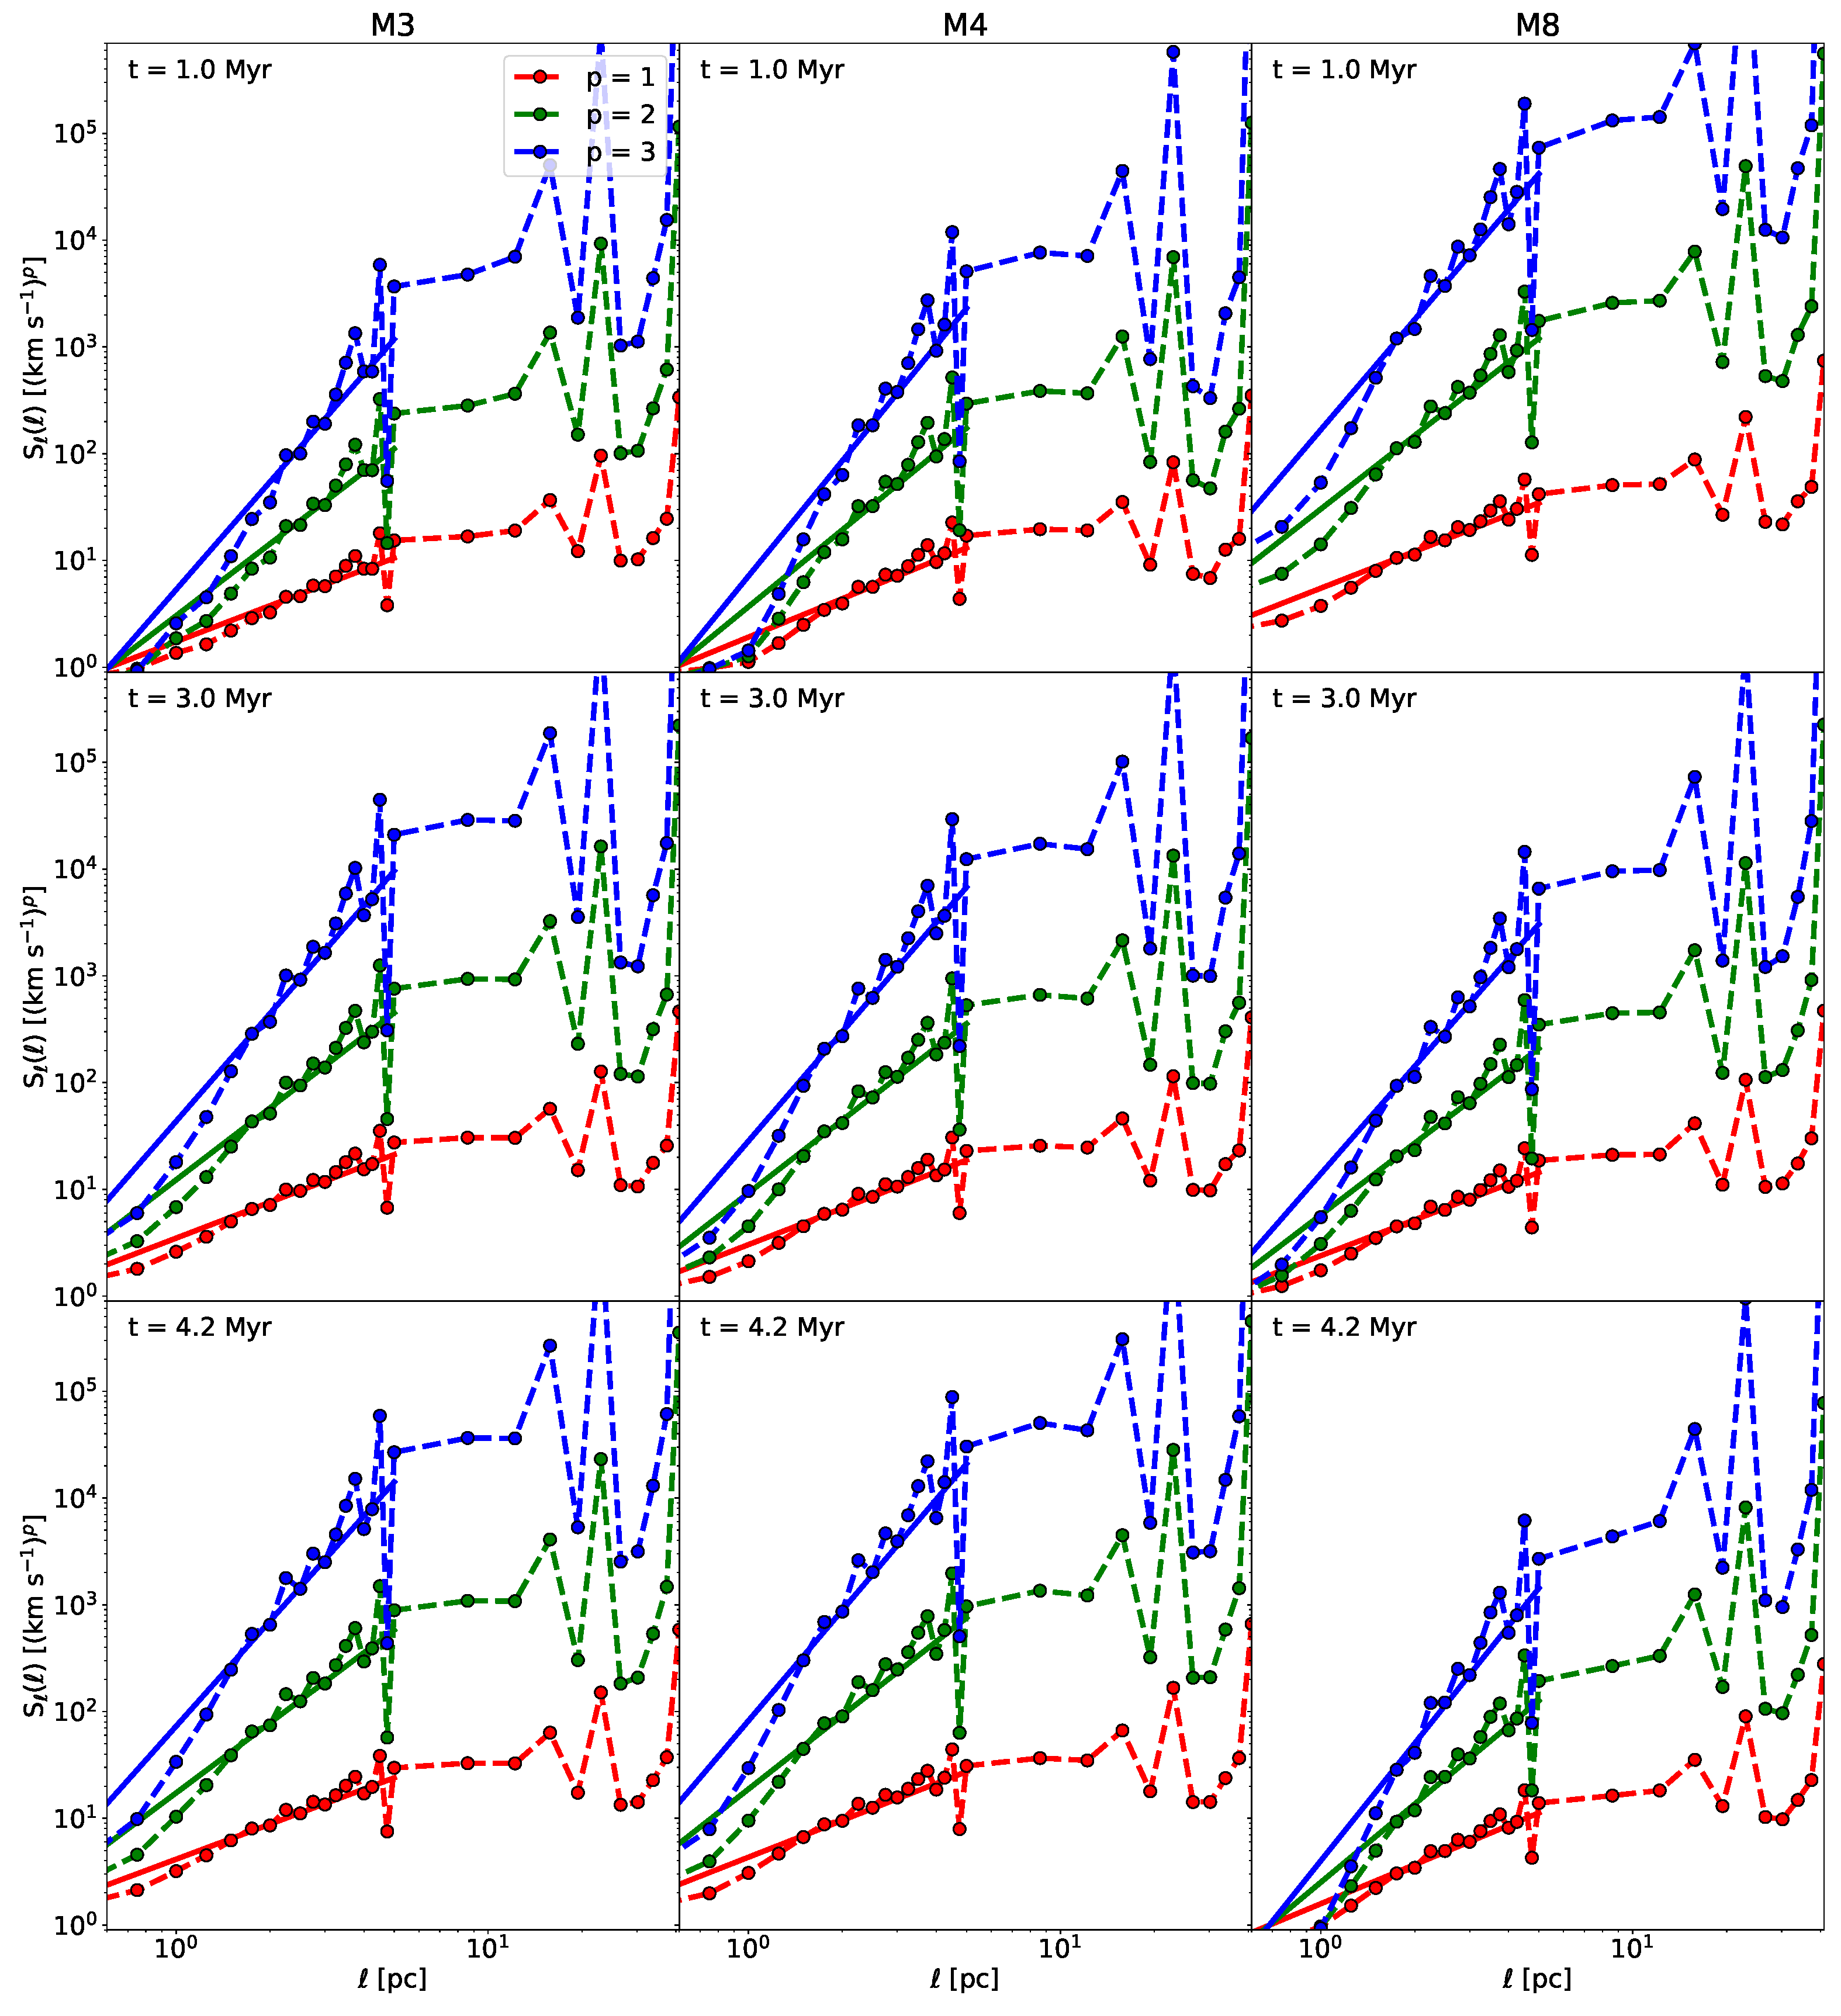
\includegraphics[width=\textwidth]{app_examples_woutthres_s_l.pdf}
    \caption{
        As Fig.~\ref{pic:appFigures:examples_with_threshold_s_vs_l}, but based on data without density threshold.
    }
    \label{pic:appFigures:examples_without_threshold_s_vs_l}
\end{figure*}
 	
 	
\begin{figure*}
    \centering
    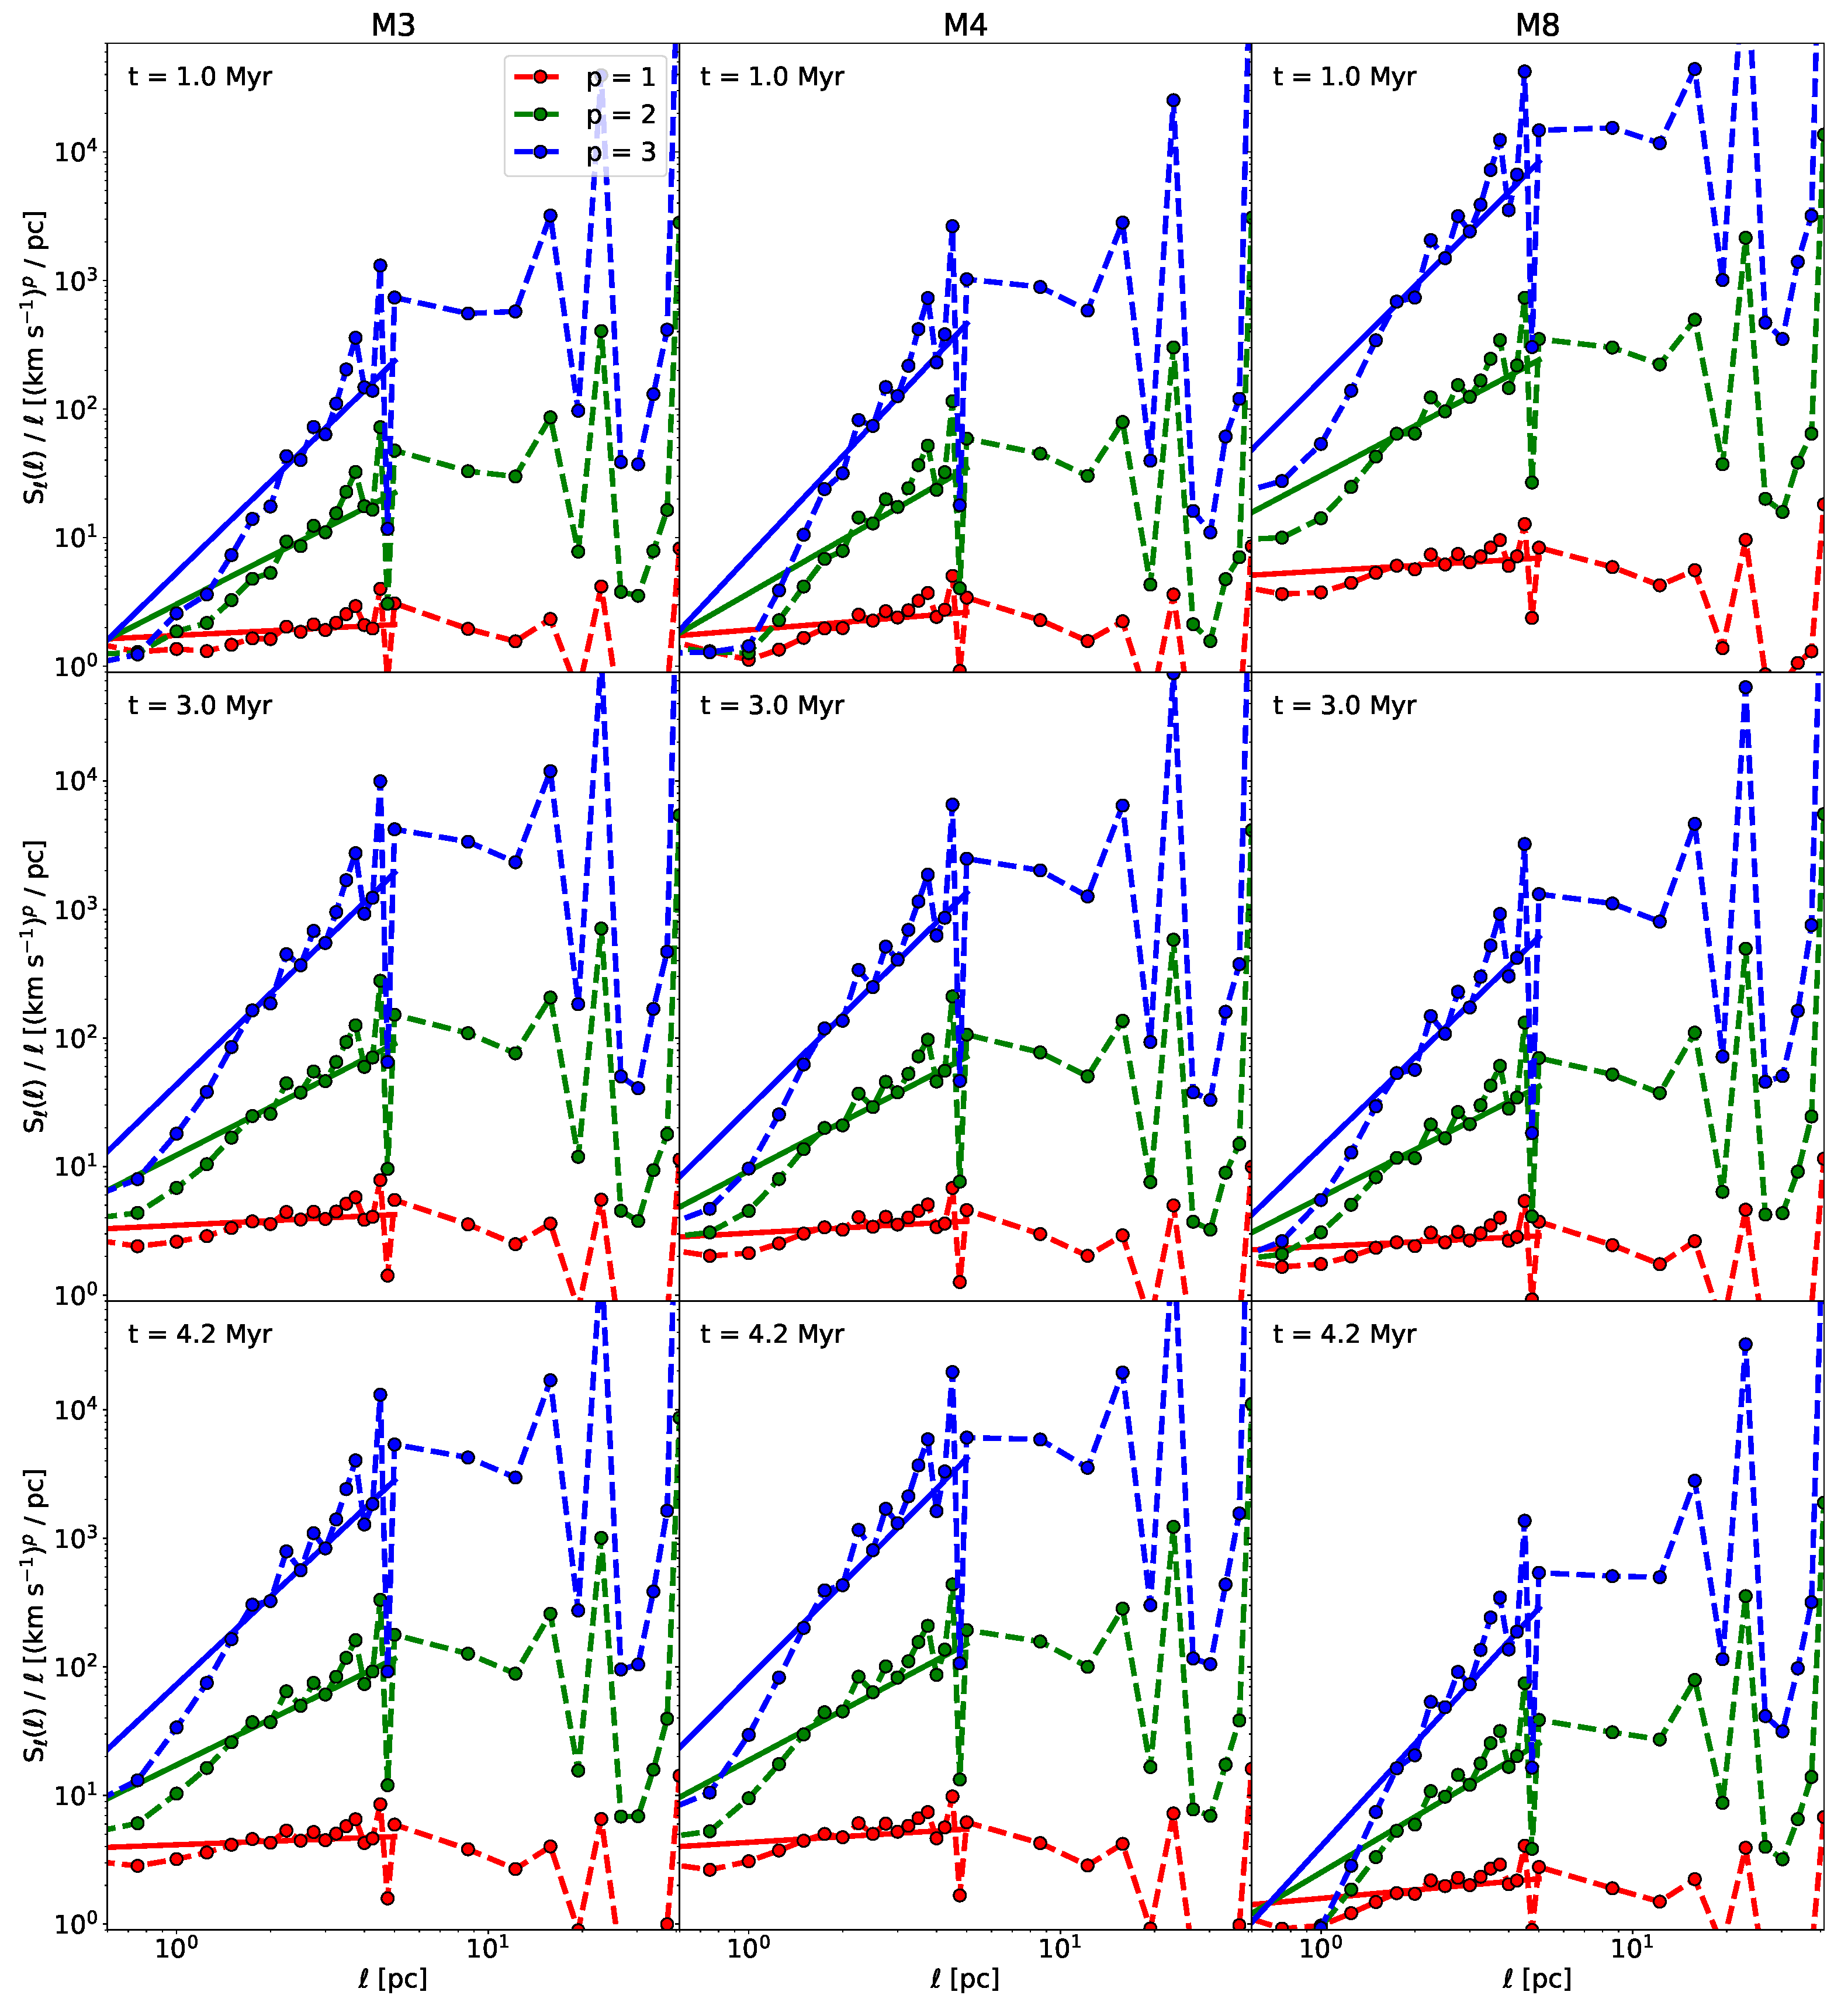
\includegraphics[width=\textwidth]{app_examples_woutthres_sl_l.pdf}
    \caption{
        As Fig.~\ref{pic:appFigures:examples_with_threshold_sl_vs_l}, but based on data without density threshold.
    }
    \label{pic:appFigures:examples_without_threshold_sl_vs_l}
\end{figure*}


 	
\begin{figure*}
    \centering
    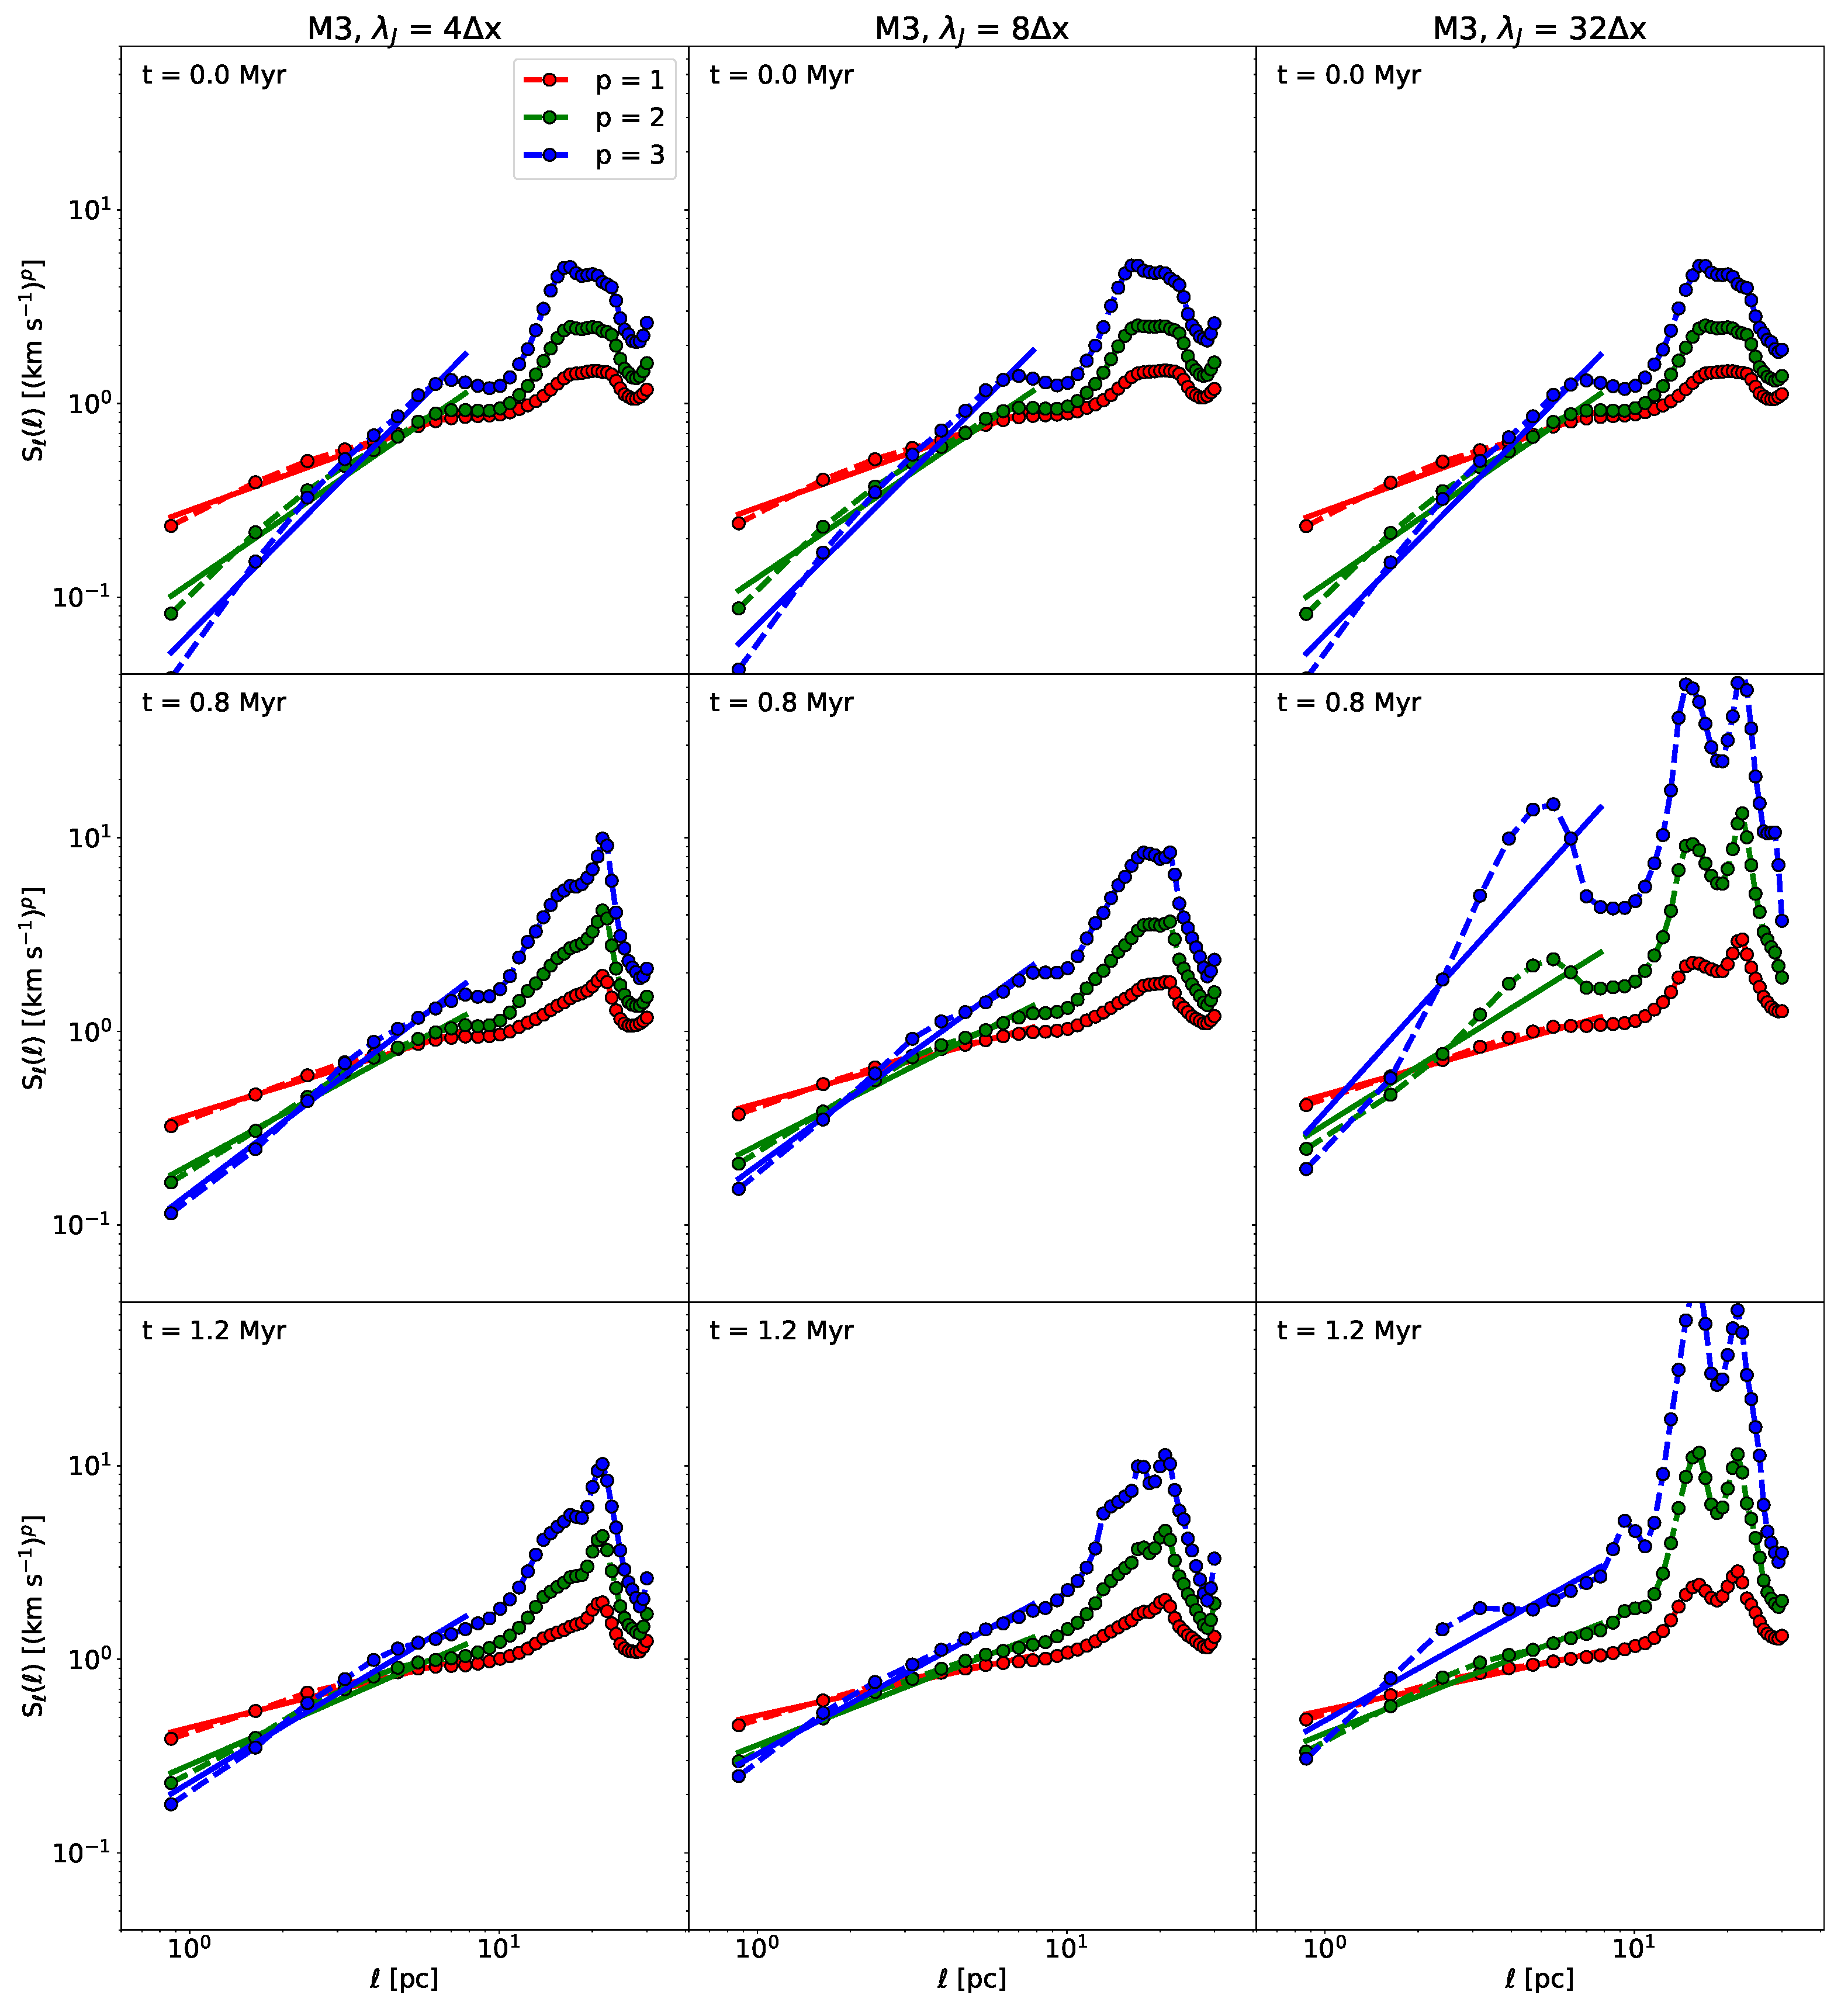
\includegraphics[width=\textwidth]{app_examples_jeans_s_l.pdf}
    \caption{
        The figures show additional examples of VSFs, based on data of \texttt{M3} with density threshold, at the different refinement levels (\textit{left} to \textit{right}) $\lambda$~=~4~$\Delta$x, $\lambda$~=~8~$\Delta$x, and $\lambda$~=~8~$\Delta$x as function of lag scale $\ell$ and order $p$. 
        The examples are given for three different time steps, namely (\textit{top} to \textit{bottom}) t~=~0.0~Myr, 0.8~Myr, and 1.2~Myr.
        The dots (connected by dashed lines) show the values computed from the simulations. 
        The solid lines represent the power-law relation fitted to the respective structure functions.
    }
    \label{pic:appFigures:examples_jeans_s_vs_l}
\end{figure*}


 	
\begin{figure*}
    \centering
    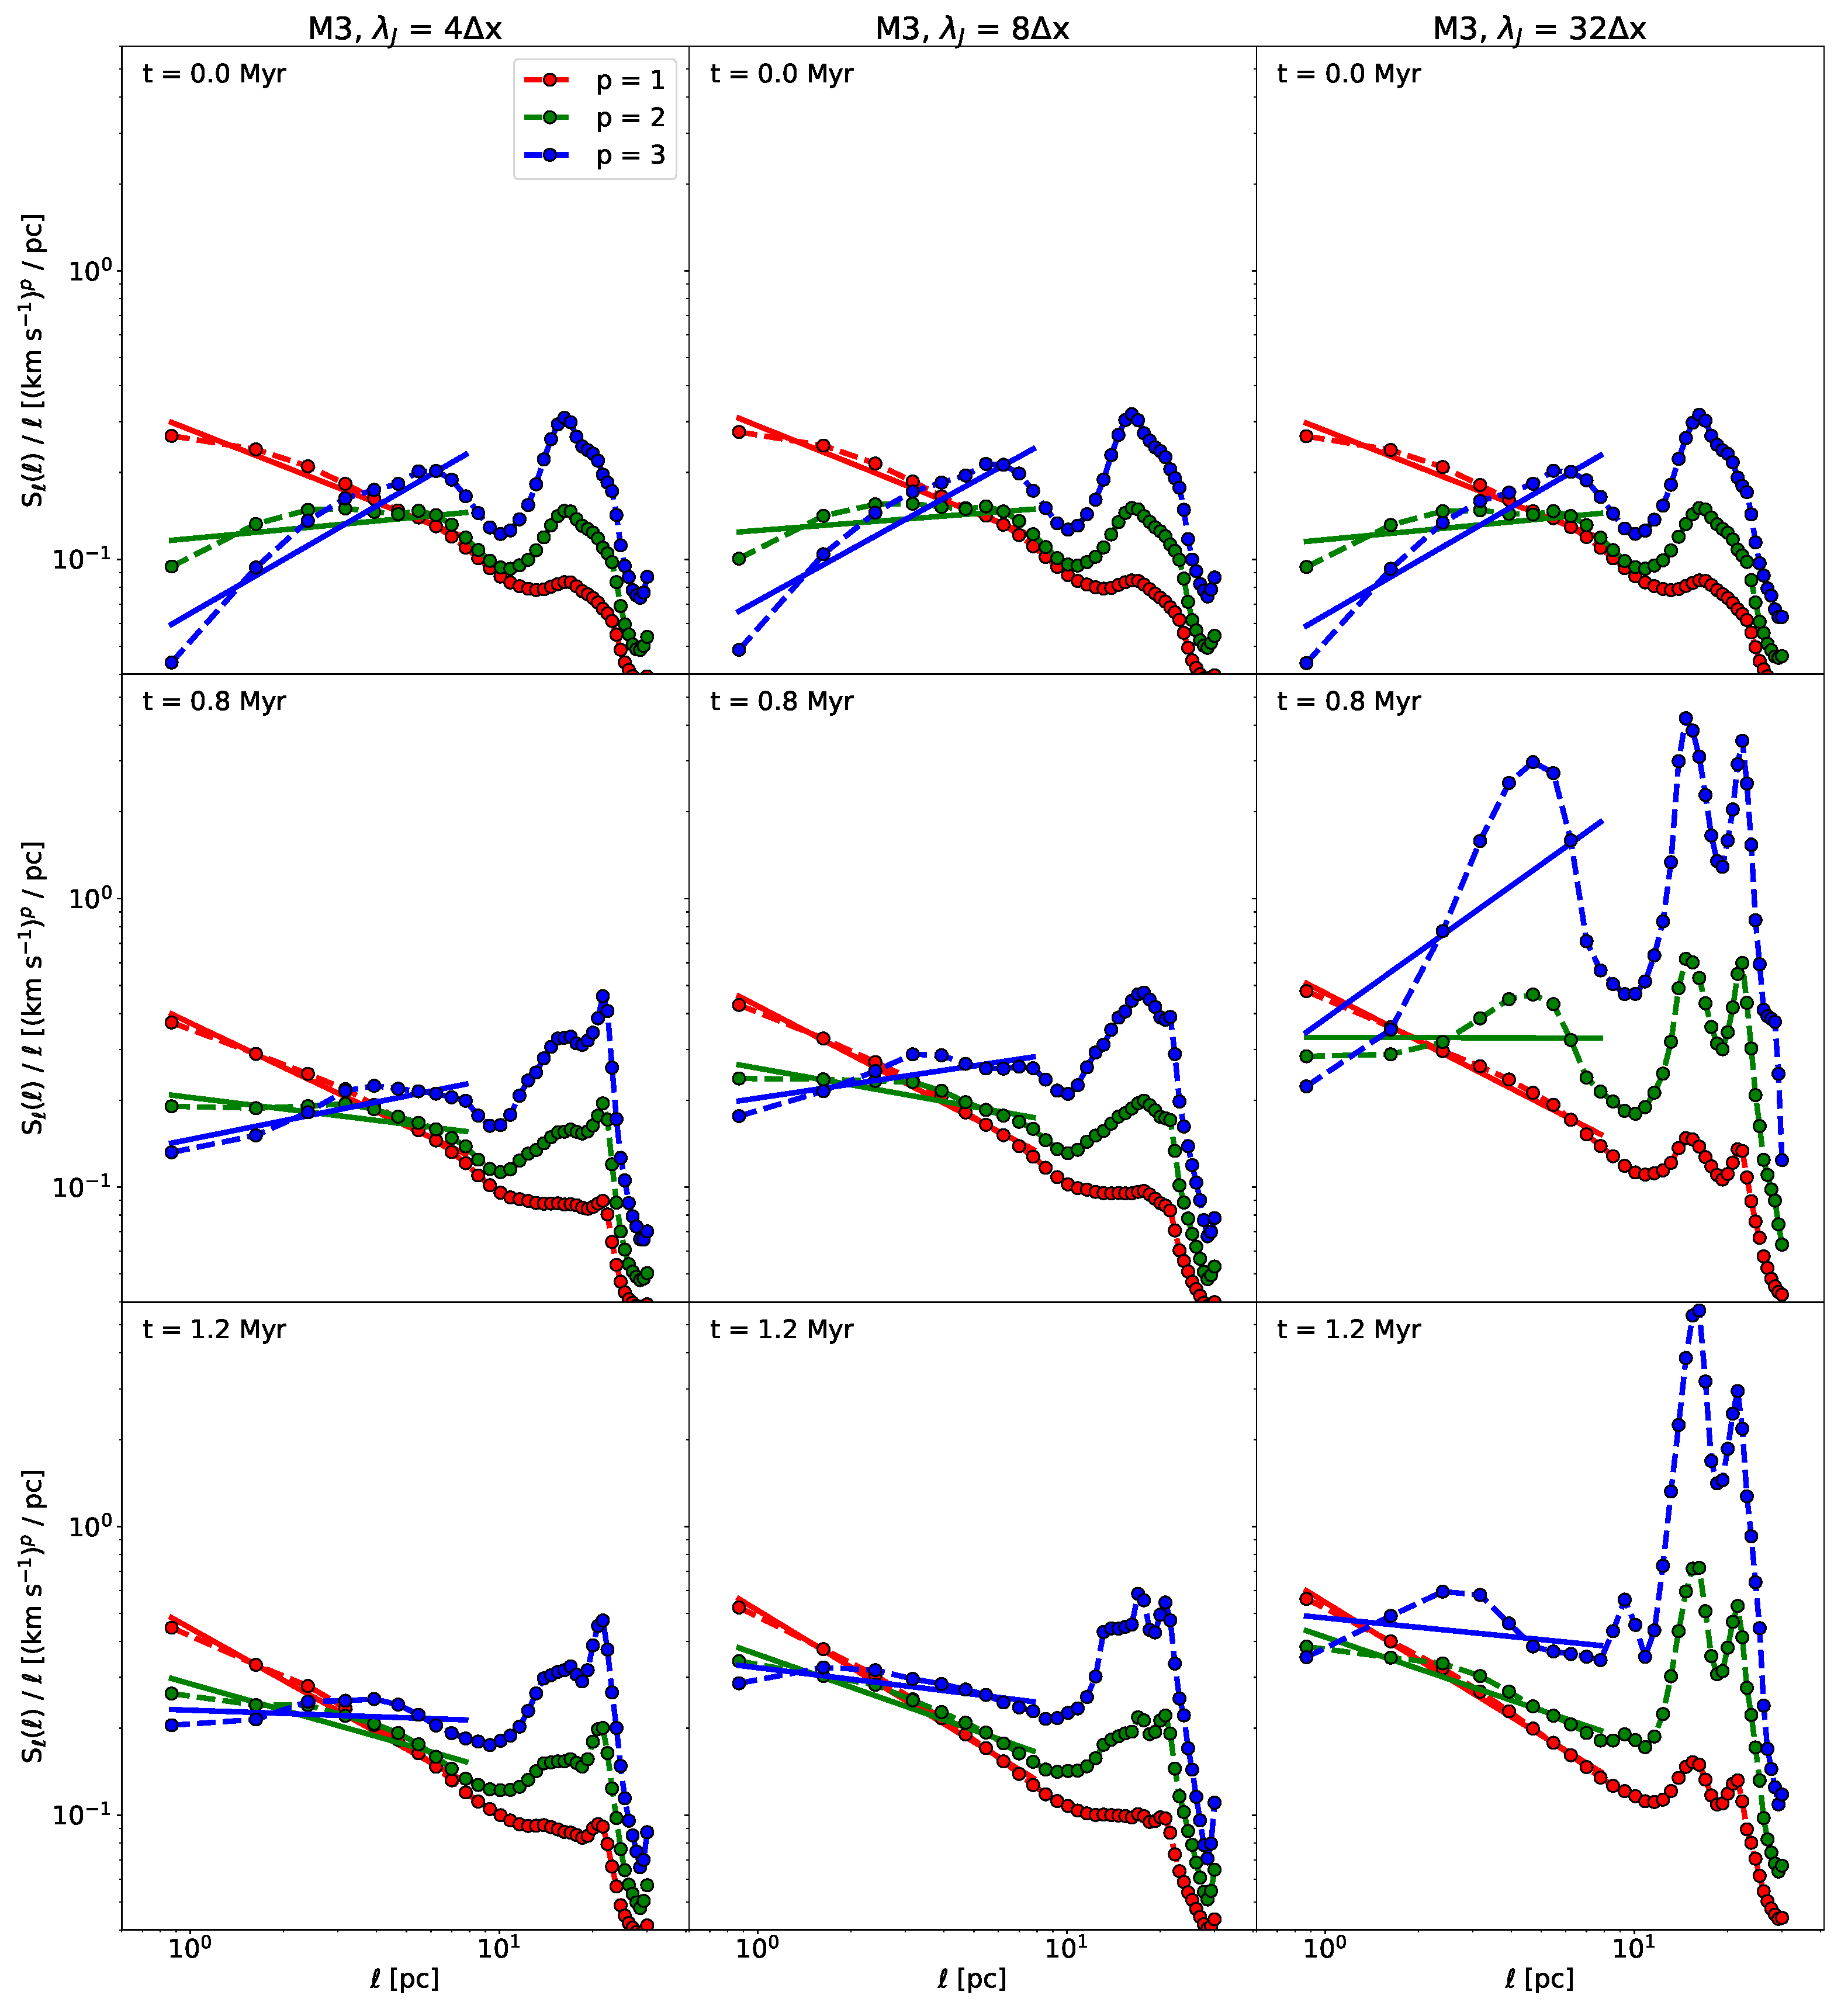
\includegraphics[width=\textwidth]{app_examples_jeans_sl_l.pdf}
    \caption{
        As Fig.~\ref{pic:appFigures:examples_jeans_s_vs_l}, but plotting the relation between S$_{\ell}$ / $\ell$ as function of lag scale $l$ and order $p$.
    }
    \label{pic:appFigures:examples_jeans_sl_vs_l}
\end{figure*}
